\documentclass{report}
\usepackage{tikz}
\usetikzlibrary{arrows,automata}
\usepackage{amsmath}
\usepackage{amssymb}
\usepackage{listings}
\setlength{\parindent}{0cm}
\lstset{language=Erlang,basicstyle=\ttfamily,columns=fixed}

\begin{document}

\title{A generic, lightweight finite state machine \\ implementation in Erlang}
\author{
   Dmitry Kolesnikov (dmkolesnikov@gmail.com) \and 
   Mario Cardona (marioxcardona@gmail.com)
}
\maketitle

%%
%%
%%
%%
\chapter{xxx}

\section{Rationale}
   The library proposes simple \emph{behaviour} for finite state machine (FSM) 
   implementation. The major objective is eliminate difference between synchronous,
   asynchronous and out-of-bound messages processing. The \emph{behaviour} is 
   proposed as an alternative to built gen\_fsm. 
  
%%
%% 
\section{Definitions}

\subsubsection{client process}
   is an Erlang process that consumes FMS services by sending \emph{synchronous}, 
   \emph{asynchronous} or \emph{out-of-bound} messages.
   
\subsubsection{finite state machine}
	is an Erlang process that executes Mealy-like FSM, which is defined as 
	the input alphabet $\Sigma$ (all acceptable messages), finite and non-empty
	set of all possible states $S$ and state transition function $\delta$ 
	(FSM output is performed at state transition).
	
	$$ \delta: x,s_i \longrightarrow s_j \quad x \in \Sigma, s \in S $$ 

\subsubsection{message}
	is an Erlang tuple used for communication between client process and FSM. 

%%
%%
\section{Message passing}
	The library distinguishes following message passing scenarios used for 
	interprocess communication. 

\subsubsection{synchronous (aka call)}
	the execution of message originator is blocked until state machine output 
	successful/unsuccessful result message. The originator process  waits for 
	response or \emph{timeout}. 	
   
\subsubsection{asynchronous (aka cast)}
	the execution of message originator is not blocked, the state machine output
	message is delivered to mailbox of originator process. The asynchronous message
	implies that originator process waits for successful/unsuccessful responses. 
	The scenario allows to execute multiple parallel service calls towards FSM 
	(e.g. asynchronous external I/O, ``long-lasting'' requests with external 
	worker pool).
 	
\subsubsection{out-of-bound (aka send)}
	the execution of message originator is not blocked, unlike an asynchronous 
	message the originator processes do not have intent to to track results of 
	service execution (fire-and-forget mode). 

	
\section{Interface specification}

%%
%%
\subsection{Data-types signatures}

\subsubsection{fsm}
	unique instance of state machine identity: $ pid | atom | any$. 

\subsubsection{ref}
	unique request reference (corresponds to Erlang built-in reference type).

\subsubsection{sid}
	$atom$ name of state transition function
	
\subsubsection{state}
	$any$ state machine internal data structure


%%
%%
\subsection{Messaging operation}
   The chapter below highlights the signatures  of message passing interface at 
   the library.

\subsubsection{call}
	the call operation sends $any$ message to the state machine and waits for 
	either $any$ successful or $any$ unsuccessful response 

	$$ call: fsm,any \longrightarrow \{'ok', any\} | \{'error', any\} $$


\subsubsection{cast}
	the cast operation sends $any$ message to the state machine and immediately 
	returns unique reference. The reference allows to asynchronously ``wait'' for
	either $any$ successful or $any$ unsuccessful response (e.g. response message 
	signature is $\{'ok' | 'error', ref, any\} $). reference generated automatically. 
	 
   $$ cast: fsm,any \longrightarrow ref$$
  

\subsubsection{send}
	the send operation does not differs from Erlang builtin ! operator or erlang:send
	function call.

	$$ send: fsm,any \longrightarrow ok$$

%%
%%
\subsection{FSM operation}
   The chapter below highlights the signatures of state machine interface at 
   the library.

\subsubsection{init}
	the function init state machine, builds internal state data $state$ and defines
	initial state (transition function) $sid$. The function is called whenever 
	state machine is started using kfsm:start\_link(...)
	
	$$ init: [any] \longrightarrow \{ok, sid, state\} | \{'error', reason\} $$
	
	

\subsubsection{free}
	the function release state machine, it is called when FSM is about to terminate. 

	$$ free: reason,state  \longrightarrow  ok $$


\subsubsection{state transition}
	the state transition function receive $any$ message, which is sent using 
	message passing interface. The function executes the state transition and 
	generates output. There should be one instance of the state transition function 
	$\delta$ for each possible state name. This function performs update of 
	internal state data, continues FSM to next state or terminates execution
	with a reason. If the input message are sent using $call$ or $cast$ primitives
	and state machine transition function do not generate any output then origin
	of input message is queued in FIFO manner for any further usage.
	
	$$\begin{array}{ll}
	\delta: any,state \longrightarrow 
	   & \{'next\_state', sid, state, [timeout | hibernate]\} \\
	   & \{'reply', any,  sid, state, [timeout | hibernate]\} \\
	   	& \{'stop', [any], reason, state\}         \\
	\end{array}$$

	$\{'next\_state', sid, state, [timeout | hibernate]\}$:
	continue execute next state $sid$ with updated internal state data $state$. 
	No output is generated to external processes by state machine. If an optional
	integer $timeout$ value is provided, a $'timeout'$ event will occur unless 
	any input is received by FSM within given time interval. If hibernate is 
	specified instead of a timeout value, the process will go into hibernation when
	waiting for the next message to arrive.\\ 
		
	$\{'reply', any,  sid, state, [timeout | hibernate]\}$:
	continue execute next state $sid$ with updated internal state data $state$. 
	The message $any$ is sent out to origin process of input message. If the origin
	is not know (e.g. pure sent or Erlang built-in functions where used) then 
	previously queued request origins are used. If the queue 
	is empty then the message $any$ is silently dropped. If an optional integer
	$timeout$ value is provided, a $timeout$ event will occur unless any input
	is received by FSM within given time interval. If hibernate is 
	specified instead of a timeout value, the process will go into hibernation when
	waiting for the next message to arrive.\\ 

	TODO: do we need a concept of subscribe here so that if origin to reply is not 
	known then subscribed process got messages (type-of-fallback scenario). \\

	$\{'stop', [any], reason, state\}$:
	terminate state machine execution with $reason$. Note that for any other reason
	than $'normal' | 'shutdown'$ FSM is assumed to terminate due to an error and 
	an error report is issued. If state machine outputs optional $any$ messages
	the it is replied to client process using same logic as previous reply scenario.
	Any outstanding synchronous calls are terminated with no\_proc exception. 
	
\subsection{OTP compatibility}

\subsubsection{gen\_server}
	gen\_server:call is translated to synchronous message passing, gen\_server:cast 
	is translated to asynchronous send. 	

\subsubsection{gen\_fsm}
	no support.

%%
%%
%%
%%
\chapter{Appendix A: Example}

\section{tcp/ip client}

	the state machine on the diagram below show a potential state machine for
	tcp/ip communication using socket api. \\\\

   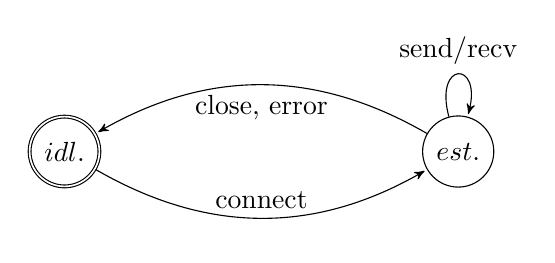
\begin{tikzpicture}[>=stealth',shorten >=1pt,auto,node distance=5cm]
   		\node[state,accepting] (I)                      {$idl.$};
		\node[state]           (E)   [right       of=I] {$est.$};
 
      \path[->]  
      		 (I) edge [bend right] node {connect}      (E)
		    (E) edge [bend right] node {close, error} (I)
			 (E) edge [loop above] node {send/recv}    (E);
   \end{tikzpicture}


\subsubsection{client interface}
   \lstinputlisting[language=Erlang]{tcp_iface.erl}

\subsubsection{tcp fsm}
   \lstinputlisting[language=Erlang]{tcp_fsm.erl}

\section{basic client-server}
   \lstinputlisting[language=Erlang]{server.erl}

   
\end{document}